\documentclass[12pt,a4paper,oneside]{erdc}
%\documentclass{erdc}
\usepackage[T1]{fontenc}		% Selecao de codigos de fonte.
\usepackage[utf8]{inputenc}		% Codificacao do documento (conversão automática dos acentos)
%\usepackage{lastpage}			% Usado pela Ficha catalográfica
\usepackage{indentfirst}		% Indenta o primeiro parágrafo de cada seção.
\usepackage{color}				% Controle das cores
\usepackage{graphicx}			% Inclusão de gráficos
%\usepackage{microtype} 			% para melhorias de justificação
\usepackage[brazil]{babel}
%\usepackage[brazilian,hyperpageref]{backref}	 % Paginas com as citações na bibl
%\usepackage[alf]{abntex2cite}	% Citações padrão ABNT
\usepackage{hyperref}
\usepackage{natbib}

\usepackage{lipsum}


\usepackage{Sweave}
\begin{document}
\Sconcordance{concordance:BP_Curso_TecComp_00_2019.tex:BP_Curso_TecComp_00_2019.Rnw:%
1 18 1 1 0 92 1 1 5 388 1}


\frontmatter

\laboratory{PPGE-UFPA}

\reportnum{BP/EcoS - Curso-DataScience-00-2019}

\program{Construção de Modelos e Indicadores Econômicos}

\title{Introdução ao Tratamento e Análise de Dados em R}

%\subtitle{Assessments and Report from Socioeconomic and Demographic Data in \\
%	      Small Cities in Amazon Delta}

\subtitle{ou Data Science para todos!}

\date{\today}

\author{S.~Rivero \and H.~Farias}

\affiliation{Programa de Pós-Graduação em Economia\\
  Instituto de Ciências Sociais Aplicadas\\
  Universidade Federal do Pará\\
  Rua Augusto Correia, 1\\
  Belém, Pará - 66.075-200}

\author{Equipe UFPA }


\affiliation{Faculdade de Economia \\
	Instituto de Ciências Sociais Aplicadas\\
	Universidade Federal do Pará\\
	Rua Augusto Correia, 1\\
	Belém, Pará - 66.075-200}


\coverart[width=\linewidth]{../figs/Capa}

\reporttype{Produto: Cursos}

\distribution{Propriedade BANPARÁ e PPGE-UFPA \\ (Distribuição Restrita)}

% \distribution{Distribution authorized to U.S. Government Agencies
% only; Test and Evaluation; November 2005.  Other requests should be
% referred to U.S. Army Engineer Research and Development Center}

%\additionalinfo{Supersedes ERDC/CREL AF-01-23}

%\begin{abstract}
%  \lipsum[12-13]
%\end{abstract}

\disclaimer{
	
	This document is an output from the  Banpará Project 
	
	PPGE-UFPA report
	
	Distribution Restrictions
	
	\copyright 2019, All rights reserved
	
	\pagebreak
	
	}

\preparedfor{Banpará} 

\contractnum{FADESP-NO-CONTRATO}

\monitoredby{Banpará}

%\preparedfor{}




\maketitle

\tableofcontents


%\chapter*{Resumo Executivo}


\mainmatter

%%%%%%%%%%%%%%%%%%%%%%%%%%%%%%%%%%%%%%%%%%%%%%%%%
%  Chamadas de Bibliotecas e Variaveis Globais
%%%%%%%%%%%%%%%%%%%%%%%%%%%%%%%%%%%%%%%%%%%%%%%%%




%%%%%%%%%%%%%%%%%%%%%%%%%%%%%%%%%%%%%%%%%%%%%%%%%%%%%%%%%
%
%    CAPITULO
%
%%%%%%%%%%%%%%%%%%%%%%%%%%%%%%%%%%%%%%%%%%%%%%%%%%%%%%%%%
%
% !Rnw root = BP_Curso_TecComp_00_2019.Rnw


\chapter*{Introdução}

O R é uma suíte integrada de software que permite a recuperação, o tratamento, e a análise de dados\cite{Venables2011}. Pode se dizer que o R é um ambiente de tratamento de dados que permite ao usuário, além a análise de dados propriamente dita, escrever extensões e ampliar o seu escopo.

R é uma ferramenta de software livre que atende aos critérios da \textit{Free Software Foundation} e tem uma licença \textbf{GNU}\footnote{\url{https://www.gnu.org/}}

Algumas das funcionalidade do R são\cite{Venables2011}:
\begin{itemize}
	\item Ferramentas para manuseio e armazenamento de dados
	\item Um conjunto de operadores que permitem o cálculo numérico e a manipulação de matrizes
	\item Um enorme conjunto de bibliotecas para análise de dados
	\item Ferramentas para apresentação gráfica de dados e resultados
	\item Uma linguagem de programação orientada a objetos e extensível
	\item A possibilidade de estender a linguagem, suas bibliotecas e funções
\end{itemize}

\begin{figure}
	\centering
	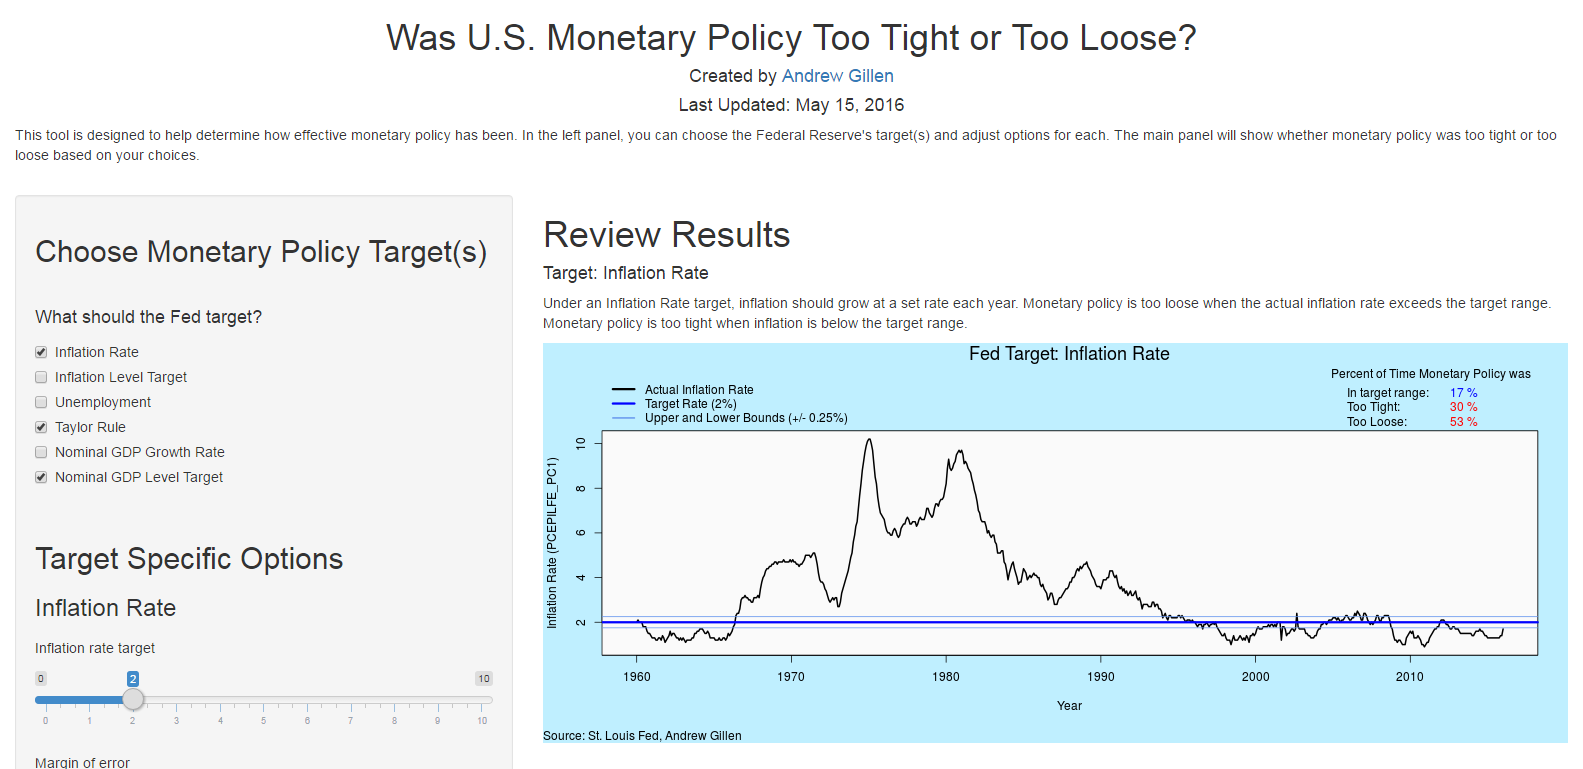
\includegraphics[width=\linewidth]{../figs/f-Intro-01-Monetary-Policy}
	\caption{Exemplo de \textit{Dashboard} de Política monetária usando R \cite{Showmeshiny2019}}
	\label{fig:f-intro-01}
\end{figure}

O R tem um conjunto extenso de ferramentas que permitem desde uma análise simples de regressão ou de aglomerados (\textit{cluster}) até apresentações de resultados extraídos de bancos de dados em larga escala com ferramentas de busca \textit{SQL}\footnote{Structured Query Language - \url{https://pt.wikipedia.org/wiki/SQL}} apresentadas em páginas web (Figura \ref{fig:f-intro-01}).

Neste texto, iremos apresentar um conjunto de ferramentas de uso livre, a sua maioria de código aberto, que permitirão a extração, tratamento, análise e apresentação de dados, tanto para análises estatísticas mais diretas quanto para a tomada de decisões estratégicas de negócios.


%%%%%%%%%%%%%%%%%%%%%%%%%%%%%%%%%%%%%%%%%%%%%%%%%%%%%%%%%
%
%    CAPITULO 1
%
%%%%%%%%%%%%%%%%%%%%%%%%%%%%%%%%%%%%%%%%%%%%%%%%%%%%%%%%%


%%%%%%%%%%%%%%%%%%%%%%%%%%%%%%%%%%%%%%%%%%%%%%%%%%%%%%%%%
%
%    CAPITULO
%
%%%%%%%%%%%%%%%%%%%%%%%%%%%%%%%%%%%%%%%%%%%%%%%%%%%%%%%%%
%
% !Rnw root = BP_Curso_TecComp_00_2019.Rnw


\chapter{Aula 1 - Instalando e Configurando o R e RStudio}


Nesta aula os alunos aprenderão a baixar o R e RStudio bem como aprenderão a utilizar bibliotecas em R


\section{Instalando o R e RStudio}

\subsection{Instalando o R}

Para instalar o R é preciso acessar o site \url{https://www.r-project.org/}. Os passos estão enumerados a seguir:

Nesta página clicar em \textbf{download R} que acessa a página - \url{https://cran.r-project.org/mirrors.html} - (Figura \ref{fig:f01-01})





\begin{figure}[htpb]
	\centering
	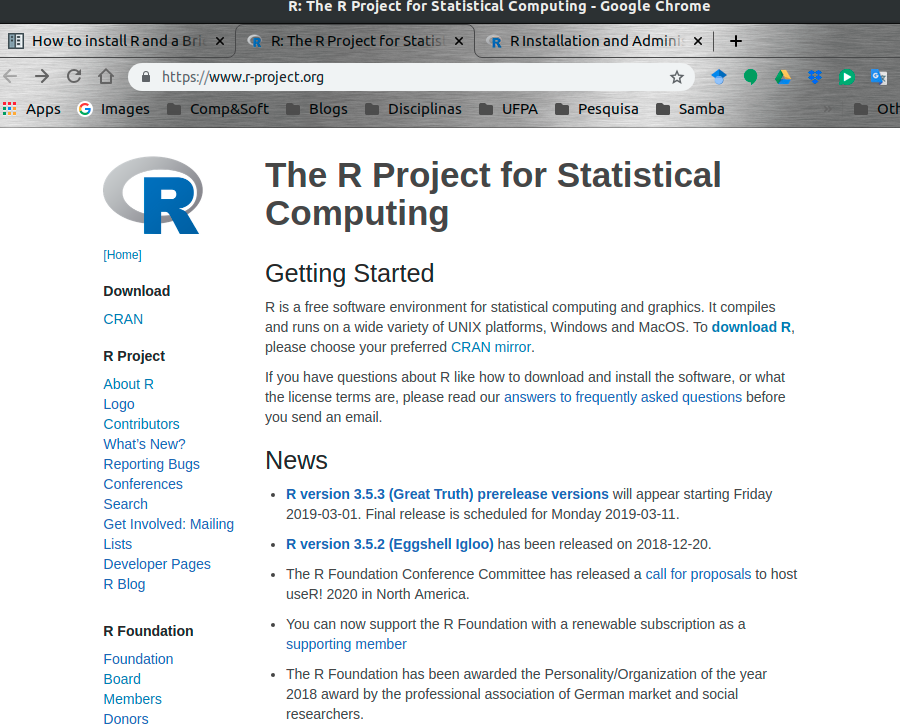
\includegraphics[width=\linewidth]{../figs/BP_Curso_TecComp_00_2019_f01-01}
	\caption{Nesta página clicar em \textbf{download R}}
	\label{fig:f01-01}
\end{figure}

Nesta página você seleciona o espelho que utilizará para baixar o R. Há sites no Brasil ou sítios em nuvem o item 0 - Cloud redirecionará automaticamente para sítios apoiados pelo Rstudio  -  \url{https://cloud.r-project.org/} (Figura \ref{fig:f01-02}) - A diferença entre os prefixos \textit{http} e \textit{https} é que os sites com \textbf{"s"} utilizam encriptação. Muitas vezes é necessário utilizar o \textit{https} em instalações cujos ambientes de TI exigem.



\begin{figure}[htpb]
	\centering
	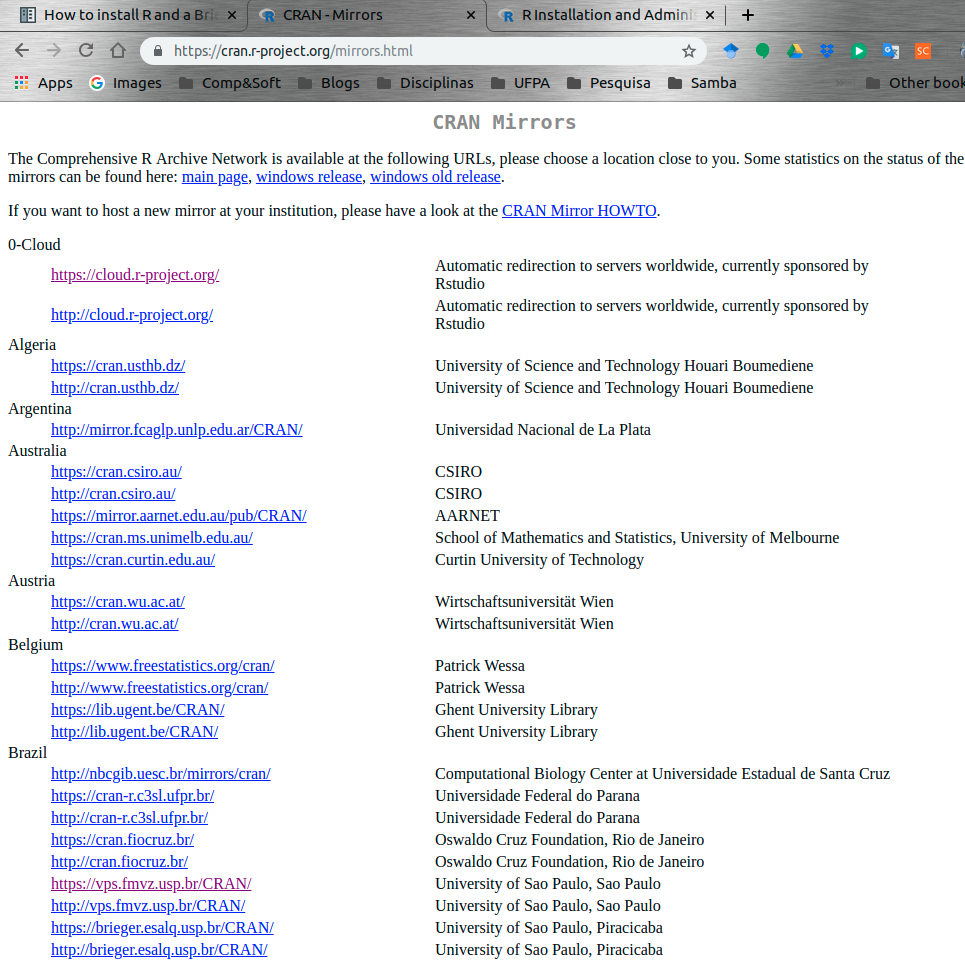
\includegraphics[width=\linewidth]{../figs/BP_Curso_TecComp_00_2019_f01-02}
	\caption{Aqui você seleciona o espelho que vai usar para baixar o R}
	\label{fig:f01-02}
\end{figure}

Você poderá baixar o R (por exemplo em \url{https://cloud.r-project.org/}) ou em algum dos outros espelhos citados anteriormente, de acordo com seu sistema operacional (Figura \ref{fig:f01-03}) Cada sistema (\textit{Linux}, \textit{MacOSX} ou \textit{Windows} tem uma rotina diferente para instalação. Aqui vamos explicar o sistema operacional mais comum (\textit{Windows}). Para outros sistemas, recomenda-se buscar instruções específicas em fóruns adequados.


\begin{figure}[htpb]
	\centering
	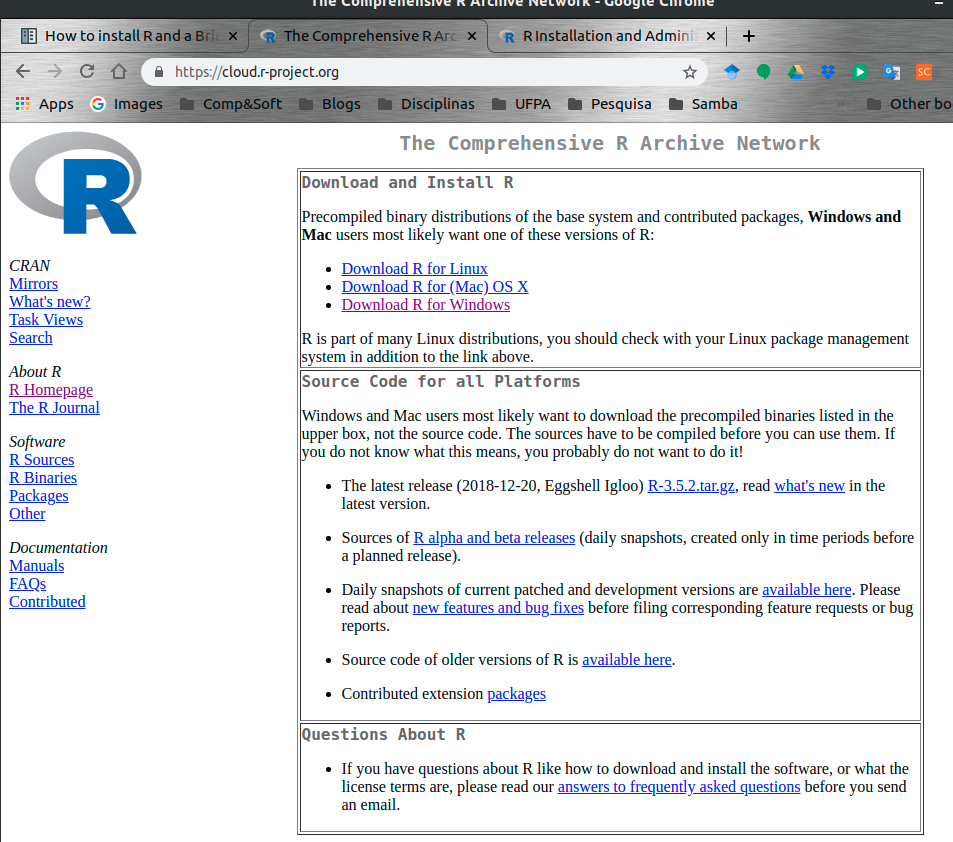
\includegraphics[width=\linewidth]{../figs/BP_Curso_TecComp_00_2019_f01-03}
	\caption{Sítio para baixar o R de acordo com seu sistema operacional}
	\label{fig:f01-03}
\end{figure}


Finalmente, para instalar o R, você pode executar o arquivo que está no link apresentado na Figura \ref{fig:f01-04}. Você baixará um arquivo \textbf{.exe} e, ao executá-lo, o instalador do \textit{Windows} tornará o programa disponível para uso na sua máquina. 

\begin{figure}[htpb]
	\centering
	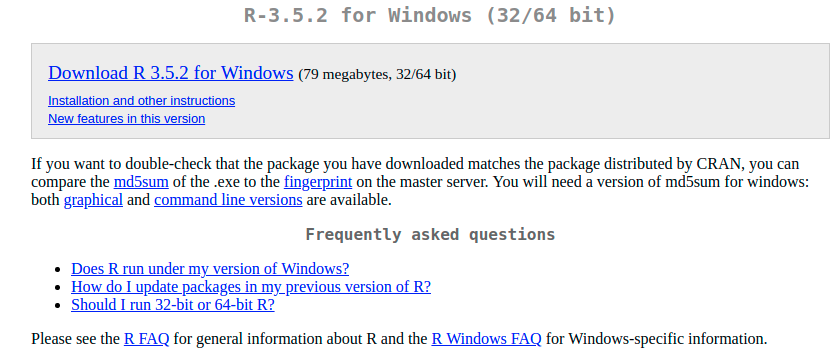
\includegraphics[width=\linewidth]{../figs/BP_Curso_TecComp_00_2019_f01-04}
	\caption{Página do Download do R}
	\label{fig:f01-04}
\end{figure}


Você pode conseguir mais informações sobre o R e os detalhes da instalação checando nos \textit{FAQs}\footnote{Frequently Asked Questions} dos sítios que você estiver acessando \url{https://cloud.r-project.org/bin/windows/base/rw-FAQ.html}, ou em \url{https://cran.r-project.org/doc/manuals/R-admin.html}



\subsection{Instalando o RStudio}

O RStudio é um ambiente de desenvolvimento integrado para o R. Incorpora um conjunto de funções que facilita o desenvolvimento de programas em R e a sua execução. O RStudio não é uma interface gráfica para a execução de rotinas do R, é um ambiente que permite implementar e executar programas. É um pacote comercial com partes de uso livre onde é necessário pagar pelos recursos extras.

\begin{figure}[htpb]
	\centering
	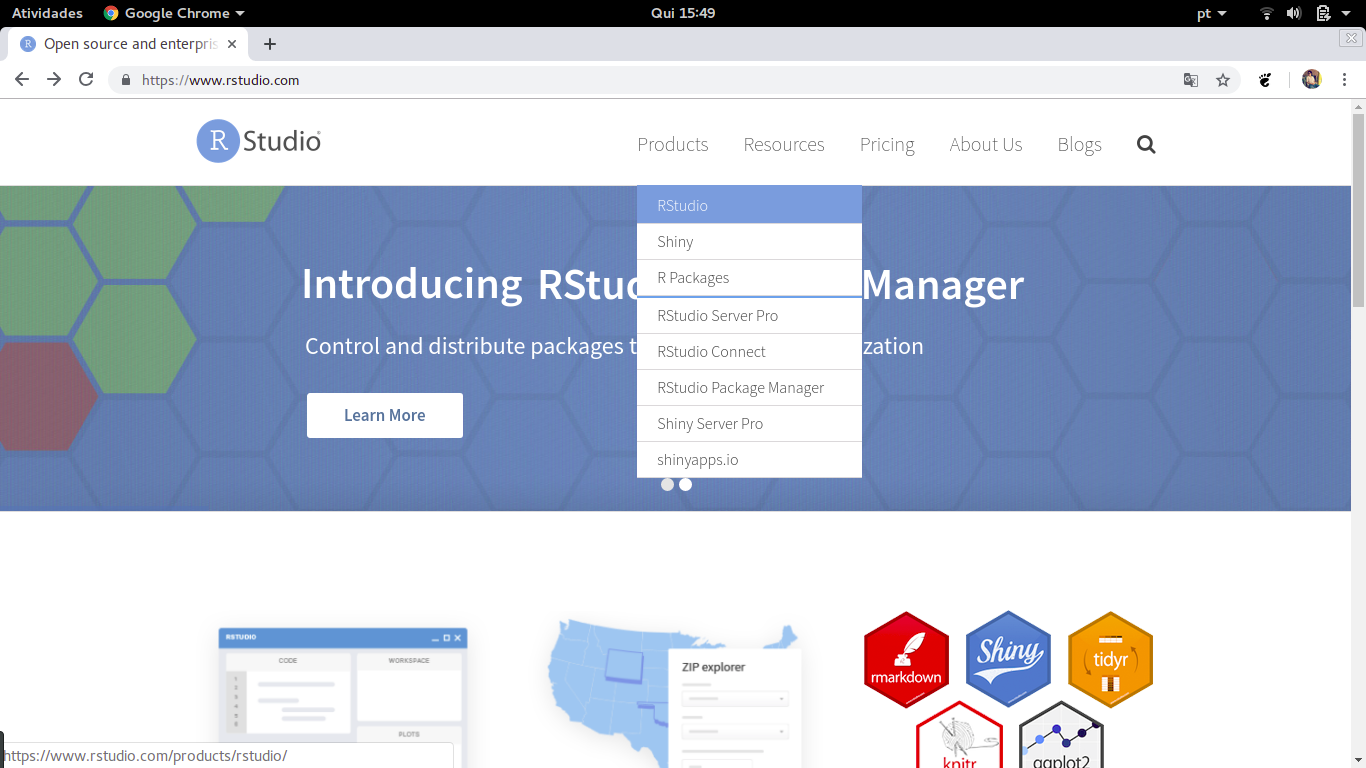
\includegraphics[width=\linewidth]{../figs/BP_Curso_TecComp_00_2019_f01-05}
	\caption{Página inicial do Rstudio}
	\label{fig:f01-05}
\end{figure}

Para iniciar o download da plataforma Rstudio é preciso acessar o site (\url{https://www.rstudio.com/}). Na parte superior há a aba \textbf{Products} que dará acesso ao item \textbf{Rstudio} como pode ser visto na figura \ref{fig:f01-05}. 

Após clicar no item \textbf{Rstudio} na aba \textbf{Products}, você será redirecionado para a página da figura \ref{fig:f01-06}. Nesta etapa é preciso clicar na opção \textbf{Rstudio Desktop}.

\newpage

\begin{figure}[htpb!]
	\centering
	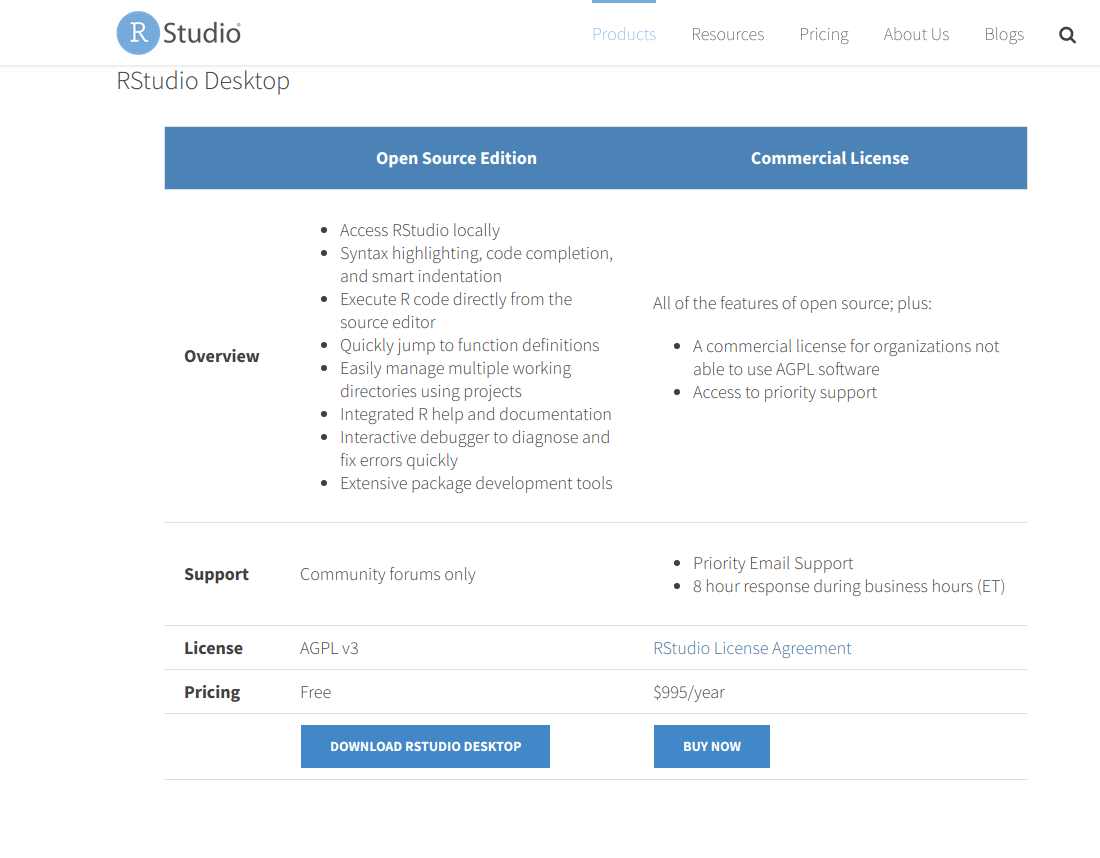
\includegraphics[width=\linewidth]{../figs/BP_Curso_TecComp_00_2019_f01-06}
	\caption{Aba de produtos do Rstudio}
	\label{fig:f01-06}
\end{figure}

\begin{figure}[htpb!]
	\centering
	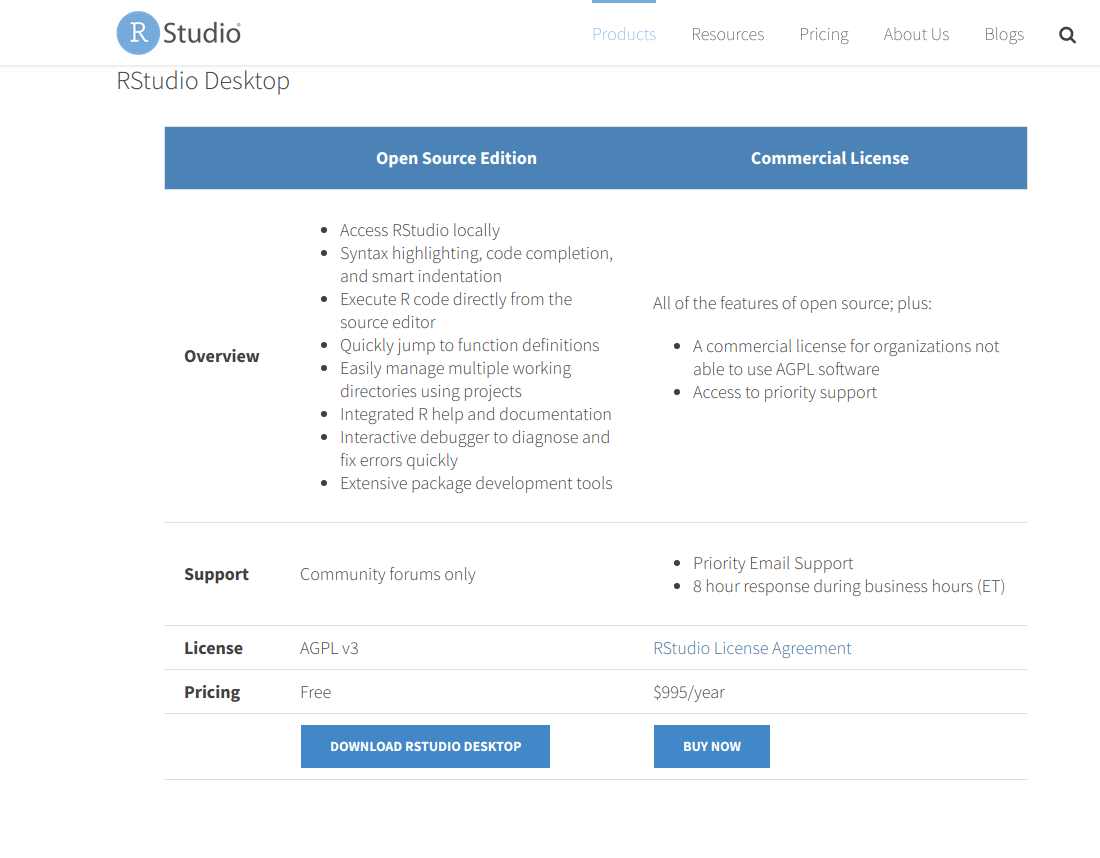
\includegraphics[width=\linewidth]{../figs/BP_Curso_TecComp_00_2019_f01-07}
	\caption{Diferença entre planos}
	\label{fig:f01-07}
\end{figure}

Após clicar em \textbf{Rstudio Desktop} na figura \ref{fig:f01-06}, será possível ter acesso a figura \ref{fig:f01-07} que mostra algumas das principais diferenças entre a plataforma de código aberto e a plataforma de licença comercial. Ainda na figura \ref{fig:f01-07}, para continuar o processo de download, é preciso clicar na aba \textbf{DOWNLOAD RSTUDIO DESKTOP}. 

Após os procedimentos da figura \ref{fig:f01-07}, você terá acesso a interface da figura \ref{fig:f01-08} que mostrará cada plano oferecido pelo \textbf{Rstudio}, bem como os benefícios e preços. O plano utilizado nesse curso será o primeiro da esquerda para direita, intulado \textbf{RStudio Desktop Open Source License}. Então para ter acesso ao download desse plano, basta clicar na respectiva aba de \textbf{download} do plano.

\begin{figure}[htpb!]
	\centering
	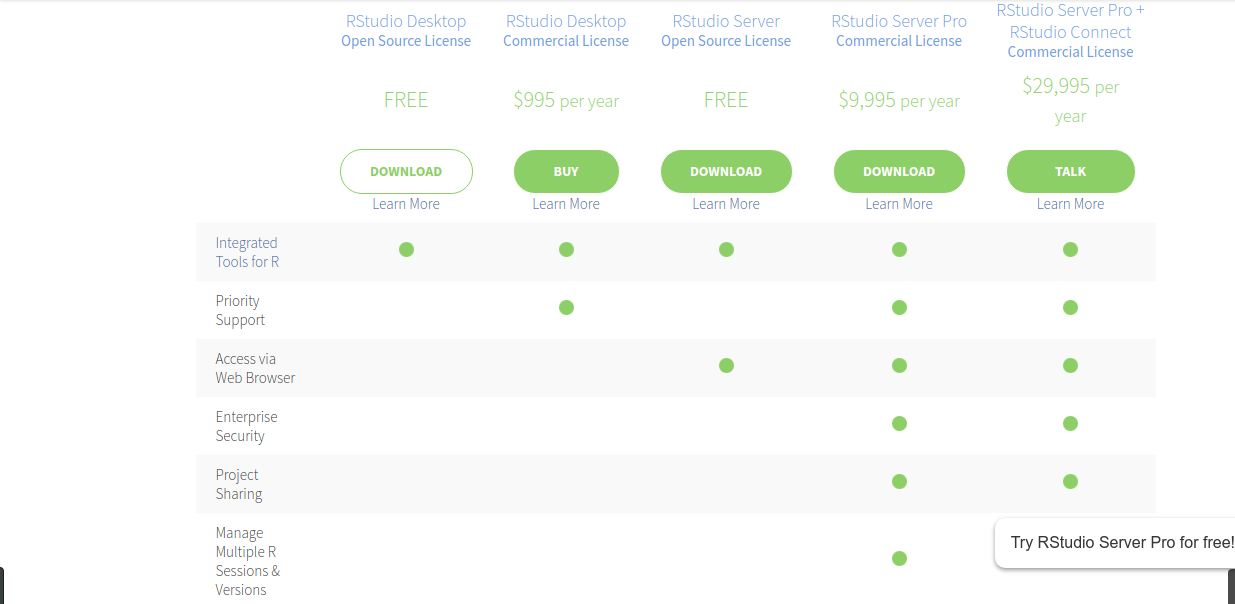
\includegraphics[width=\linewidth]{../figs/BP_Curso_TecComp_00_2019_f01-08}
	\caption{Planos, preços e benefícios}
	\label{fig:f01-08}
\end{figure}

Por fim, após os passos da figura \ref{fig:f01-08}, basta escolher o sistema operacional conforme a figura \ref{fig:f01-09}

\begin{figure}[htpb!]
	\centering
	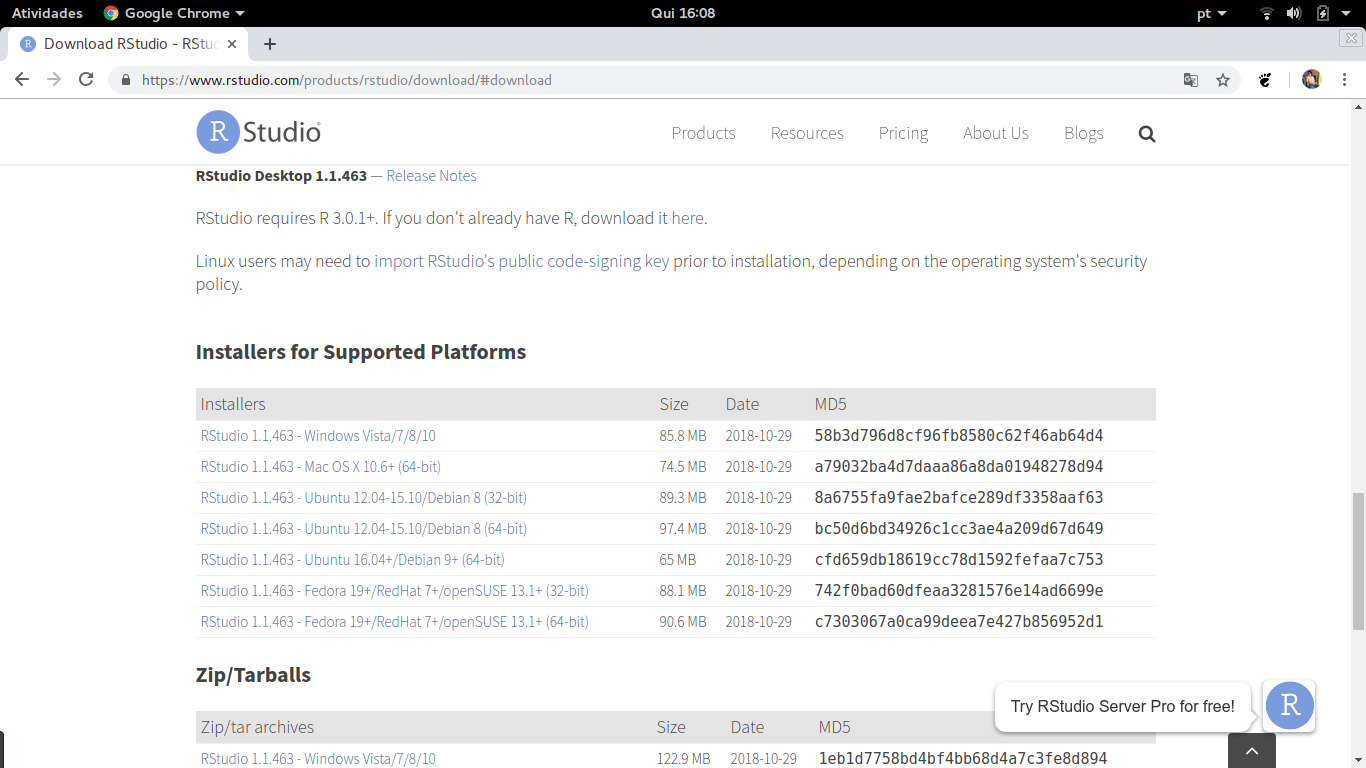
\includegraphics[width=\linewidth]{../figs/BP_Curso_TecComp_00_2019_f01-09}
	\caption{Fim! Escolha o sistema operacional}
	\label{fig:f01-09}
\end{figure}

Após o download basta executar o arquivo \textbf{RStudio-1.1.463.exe} e fazer a instalação padrão.

\section{Checando a Instalação Existente e os Requisitos}

Muitas vezes é possível que você já tenha uma versão do R e do RStudio instaladas. Um problema que pode ocorrer é você não ter a última versão do programa. Caso você já tenha o r instalado, é uma boa estratégia atualizar os pacotes para a nova versão (falaremos de pacotes na seção \ref{sec:Pacotes}).

Para checar a instalação do R você pode executar o seguinte comando:

\begin{Schunk}
\begin{Sinput}
> sessionInfo()
\end{Sinput}
\begin{Soutput}
R version 3.5.3 (2019-03-11)
Platform: x86_64-pc-linux-gnu (64-bit)
Running under: Ubuntu 18.04.2 LTS

Matrix products: default
BLAS: /usr/lib/x86_64-linux-gnu/openblas/libblas.so.3
LAPACK: /usr/lib/x86_64-linux-gnu/libopenblasp-r0.2.20.so

locale:
 [1] LC_CTYPE=pt_BR.UTF-8       LC_NUMERIC=C              
 [3] LC_TIME=pt_BR.UTF-8        LC_COLLATE=en_US.UTF-8    
 [5] LC_MONETARY=pt_BR.UTF-8    LC_MESSAGES=en_US.UTF-8   
 [7] LC_PAPER=pt_BR.UTF-8       LC_NAME=C                 
 [9] LC_ADDRESS=C               LC_TELEPHONE=C            
[11] LC_MEASUREMENT=pt_BR.UTF-8 LC_IDENTIFICATION=C       

attached base packages:
[1] stats     graphics  grDevices utils     datasets  methods   base     

other attached packages:
[1] knitr_1.21

loaded via a namespace (and not attached):
[1] compiler_3.5.3 tools_3.5.3    xfun_0.4      
\end{Soutput}
\begin{Sinput}
> 
\end{Sinput}
\end{Schunk}


O comando dará as informações da versão, plataforma, Bibliotecas, e Locales\footnote{Os \textit{Locales} dão detalhes sobre a codificação de caracteres, data, moeda, etc...}




\section{Pacotes no R}
\label{sec:Pacotes}

A maior parte da funcionalidade existente no R é fornecida pro programas, funções e bibliotecas agrupadas em pacotes. Estes pacotes são, em boa parte, resultado do esforço colaborativo de milhares de pesquisadores e entusiastas no mundo. Estes pesquisadores desenvolvem e compartilham estes pacotes na CRAN \footnote{The Comprehensive R Archive Network \\ \url{https://cran.r-project.org/web/packages/index.html}}. Lá você pode encontrar, entre os mais de 13 mil pacotes existentes, aquilo que  provavelmente vai resolver seu problema.

\subsection{O conceito de pacote e para que serve}

Um pacote em R é um conjunto de funções e arquivos de dados (\textit{Datasets}), desenvolvido pela comunidade do R e que amplia o conjunto de funcionalidades do software. Pacotes executam funções específicas (como determinados tipos de funções estatísticas) ou mesmo todo um conjunto de funcionalidades para tarefas mais gerais, como produção de gráficos (ggplot2) ou tratamento de dados (dplyr e tidyr).\footnote{
\url{https://www.datacamp.com/community/tutorials/r-packages-guide}\\
\url{https://www.rstudio.com/products/rpackages/}}

uma boa introdução sobre desenvolvimento, estrutura, e implementação de pacotes em R pode ser encontrada em \url{http://r-pkgs.had.co.nz/}.


\subsection{Como sei que pacotes eu preciso?}

Há uma profusão enorme de pacotes no R. Em geral há um padrão de documentação nos pacotes que permitem ao usuário compreender a finalidade e a forma de uso do pacote. Alguns pacotes mais difundidos, como o \textit{ggplot2} e o \textit{xtable}. Coisas mais específicas, porém, como algoritmos genéticos (\textit{ga}, \textit{genalg}) ou escores de propensão (\textit{MatchIt}) precisam ser encontradas a partir do domínio específico que se precisa.

Uma boa pedida é usar numa ferramenta de busca específica com termos como \textit{a função que eu quero} em R. (A busca em inglês é bem mais eficiente e dera mais resultados).



\begin{figure}
	\centering
	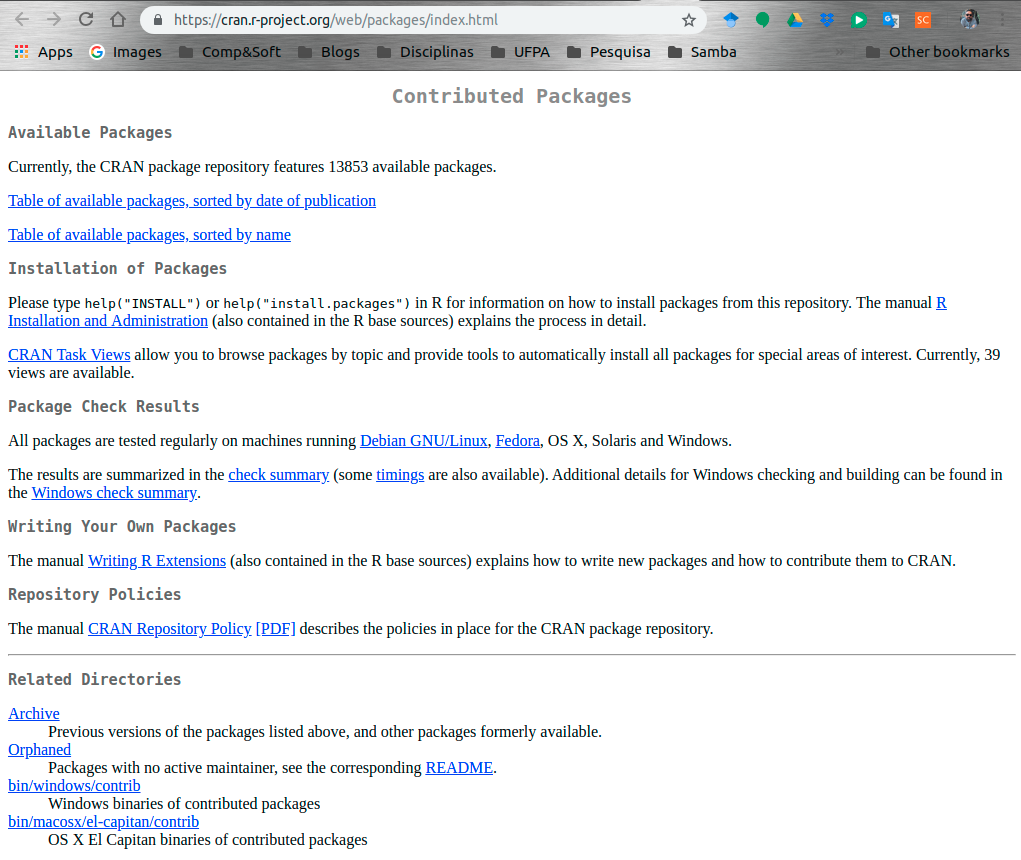
\includegraphics[width=\linewidth]{../figs/BP_Curso_TecComp_00_2019_f01-10.png}
	\caption{Página dos Pacotes Mantidos por pessoas que contribuem com o R (CRAN)}
	\label{fig:bpcursoteccomp002019f01-10}
\end{figure}


Mais informações podem ser encontradas abaixo:
\begin{itemize}
	\item \url{https://blog.revolutionanalytics.com/2017/01/cran-10000.html}
	
	\item \url{https://cran.r-project.org/web/packages/available_packages_by_name.html}
	
	\item \url{https://cran.r-project.org/web/packages/}
	
\end{itemize}


Além do \textit{CRAN}\footnote{\url{https://cran.r-project.org/}}, uma outra fonte importante para programas no R é o \textit{GitHub}\footnote{\url{https://github.com/}}. Para utilizar o \textit{GitHub}, porém, é necessário baixar o pacote \textit{devtools}. Na seção \ref{section:baixandoPacotes}, falaremos mais sobre baixar e instalar pacotes no R.



\subsection{Baixando os pacotes}
\label{section:baixandoPacotes}

O R provê uma maneira de baixar os pacotes diretamente do terminal de linha de comando. É o comando \textit{install.packages}. Abaixo, um exemplo:

\begin{Schunk}
\begin{Sinput}
> install.packages("ggplot2")
> library(ggplot2)
\end{Sinput}
\end{Schunk}

\
Acima está o exemplo de instalação do pacote \textit{ggplot2} utilizando o R na linha de comando. O mesmo pacote, instalado via RStudio está no exemplo abaixo (figura \ref{fig:bpcursoteccomp002019f01-11}) 


\begin{figure}[htpb]
	\centering
	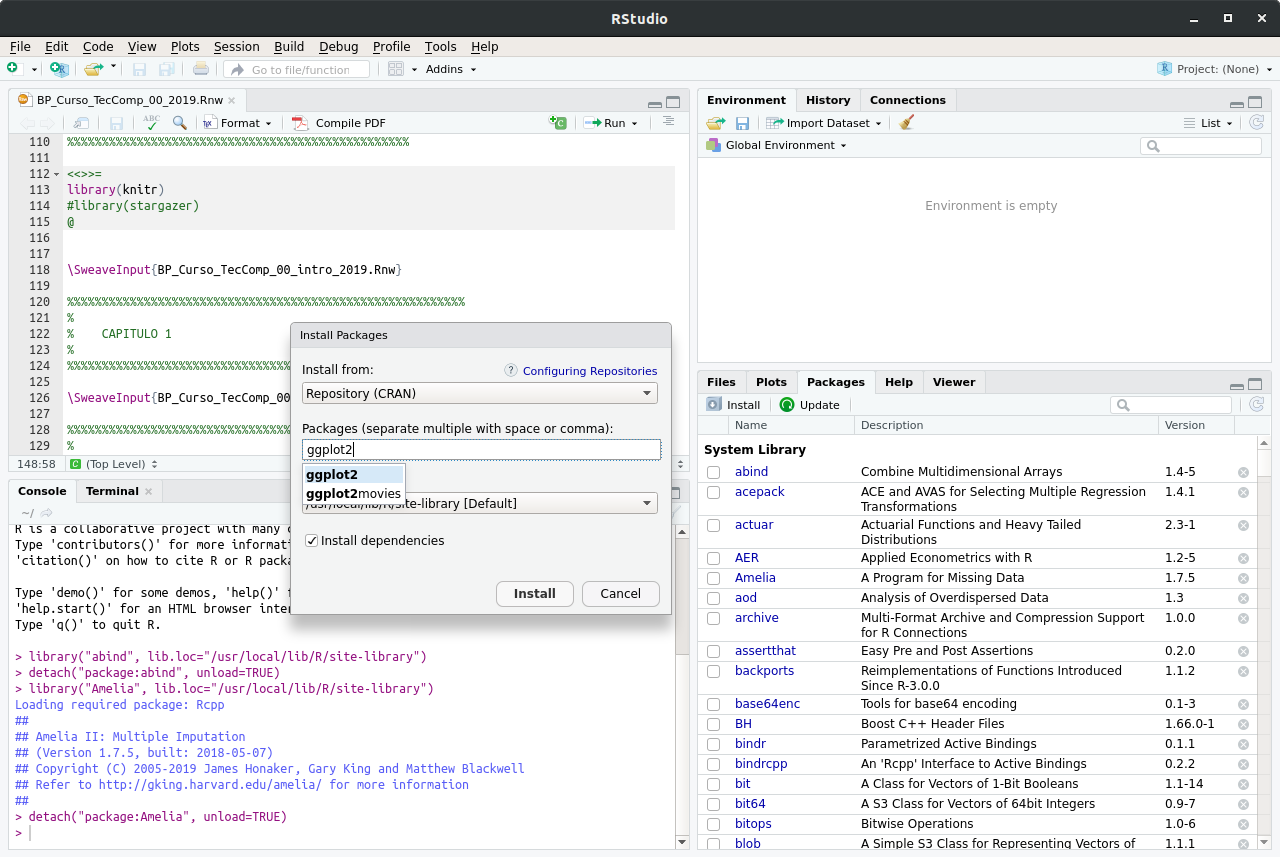
\includegraphics[width=\linewidth]{../figs/BP_Curso_TecComp_00_2019_f01-11.png}
	\caption{Instalando o pacote ggplot2 via Rstudio}
	\label{fig:bpcursoteccomp002019f01-11}
\end{figure}

Para utilizar o pacote é necessário disponibilizá-lo na seção do R que você está executando. Isto é feito com o comando \textit{library(nomeDoPacote)}.


Para o \textit{GitHub}, algum pacote específico para acessar o site deve ser instalado, o mais comum é o \textit{devtools()}. Utilizando o \textit{devtools} é possivel acessar pacotes que não estão no CRAN. 

Você pode encontrar mais informações sobre o assunto em:

\begin{itemize}
	\item \url{https://www.r-bloggers.com/installing-r-packages/}
	
	\item \url{https://www.r-bloggers.com/how-to-install-and-include-an-r-package/}
	
	\item \url{http://kbroman.org/pkg_primer/pages/build.html}
	
\end{itemize}


Para a instalação de pacotes a partir do \textit{GitHub} você pode utilizar o pacote devtools. Há outros pacotes disponíveis, mas o \textit{devtools} é o mais utilizado no momento.

\begin{Schunk}
\begin{Sinput}
> install.packages("devtools")
> library(devtools)
\end{Sinput}
\end{Schunk}

Depois de instalar a biblioteca é possível fazer uso do pacotes R disponíveis no \textit{GitHub}. Depois do pacote instalado e a biblioteca ativada no R, você pode baixar os pacotes do github com os seguintes comandos.

\begin{Schunk}
\begin{Sinput}
> install_github("DeveloperName/PackageName")
> githubinstall("PackageName")
\end{Sinput}
\end{Schunk}

O primeiro \textit{install\_github()} instala o pacote a partir do nome do usuário github, mais o nome do pacote, o segundo \textit{githubinstall()} o faz a partir do nome do pacote.

Há alguns pacotes que estão no \textit{GitHub} e no \textbf{CRAN}, a diferença é que, em geral, no \textit{GitHub} a verão acessível é a mais recente ou  de desenvolvimento. A desvantagem é que os pacotes do \textit{GitHub}, como são versões de desenvolvimento, podem, eventualmente ter problemas.

Algumas boas fontes de pacotes do \textit{GitHub} são:

\begin{itemize}
	\item \url{https://github.com/trending/r}
	\item \url{https://github.com/hadley}
\end{itemize}



\subsection{Resolvendo problemas de compilação}

\url{https://stackoverflow.com/questions/23135703/package-install-error-compilation-failed}

\url{https://support.rstudio.com/hc/en-us/community/posts/200522573-Can-t-install-packages}

\url{http://mazamascience.com/WorkingWithData/?p=1185}


\subsection{Utilizando os pacotes no seu programa R}

\url{https://www.statmethods.net/interface/packages.html}

\url{https://www.dummies.com/programming/r/how-to-install-load-and-unload-packages-in-r/}






%%%%%%%%%%%%%%%%%%%%%%%%%%%%%%%%%%%%%%%%%%%%%%%%%%%%%%%%%
%
%    CAPITULO 2
%
%%%%%%%%%%%%%%%%%%%%%%%%%%%%%%%%%%%%%%%%%%%%%%%%%%%%%%%%%


%%%%%%%%%%%%%%%%%%%%%%%%%%%%%%%%%%%%%%%%%%%%%%%%%%%%%%%%%
%
%    CAPITULO
%
%%%%%%%%%%%%%%%%%%%%%%%%%%%%%%%%%%%%%%%%%%%%%%%%%%%%%%%%%
%
% !Rnw root = BP_Curso_TecComp_00_2019.Rnw


		
\chapter{Aula 2 - Acessando e Utilizando Bases de Dados}

Apresentar o conceito de Dataframe, os tipos de dados utilizados no R e os principais comandos  

\section{O ciclo de tratamento e análise de dados}

\section{Tipos de Dados em R}

Os tipos de dados do R incluem: dados escalares, vetores, matrizes, listas e quadro de dados.

\subsection{Escalares}
Determinada variável pode ser um escalar, ou seja, simplesmente um número:

Exemplo de escalares:
\begin{Schunk}
\begin{Sinput}
> a <- 2
> b <- 2*a
> a
\end{Sinput}
\begin{Soutput}
[1] 2
\end{Soutput}
\begin{Sinput}
> b
\end{Sinput}
\begin{Soutput}
[1] 4
\end{Soutput}
\end{Schunk}

\subsection{Vetores}
O vetor é um objeto matemático caracterizado em um conjunto de segmentos orientdos de reta que possuem o mesmo módulo, direção e sentido. Ele contêm elementos de classes diferentes, conforme apresentado abaixo:


Vetor de classe numérica:
\begin{Schunk}
\begin{Sinput}
> a <- c(1,3500,5.3,543,-2,4000)
\end{Sinput}
\end{Schunk}
Vetor de classe de caractér:
\begin{Schunk}
\begin{Sinput}
> b <- c("taxa de juros","taxa de câmbio","reservas bancárias") 
\end{Sinput}
\end{Schunk}
Vetor de classe lógica:
\begin{Schunk}
\begin{Sinput}
> c <- c(FALSE,TRUE,FALSE,TRUE) 
\end{Sinput}
\end{Schunk}
\subsection{Matrizes}
São compostas por linhas (valores ordenados na horizontal) representadas pela letra "m" e colunas (valores ordenados na vertical) representadas pela letra "n", onde os dados são convertidos segundo essas disposições.
\begin{Schunk}
\begin{Sinput}
> matriz <- matrix(data=1:16,nrow=4,ncol=4)
> matriz
\end{Sinput}
\begin{Soutput}
     [,1] [,2] [,3] [,4]
[1,]    1    5    9   13
[2,]    2    6   10   14
[3,]    3    7   11   15
[4,]    4    8   12   16
\end{Soutput}
\end{Schunk}
Onde:
       \begin{description}
       \item [data:] parâmetro que representa os dados usados para criar matriz;
       \item [nrow:] parâmetro para número de linhas;
       \item [ncol:] parâmetro para número de colunas.
       \end{description}

\subsection{Array}

O dado pode ser um \textbf{Array}. Essa estrutura de dados possui três dimensões, as linhas, as colunas e as camadas. 

Exemplo de Array:
\begin{Schunk}
\begin{Sinput}
> cubo <- array(data = 1:27, dim=c(3,3,3))
> cubo
\end{Sinput}
\begin{Soutput}
, , 1

     [,1] [,2] [,3]
[1,]    1    4    7
[2,]    2    5    8
[3,]    3    6    9

, , 2

     [,1] [,2] [,3]
[1,]   10   13   16
[2,]   11   14   17
[3,]   12   15   18

, , 3

     [,1] [,2] [,3]
[1,]   19   22   25
[2,]   20   23   26
[3,]   21   24   27
\end{Soutput}
\end{Schunk}

       \begin{description}
       \item [data:] parâmetro que representa os dados usados para criar matriz;
       \item [dim:] parâmetro para determinar as dimensões do array, sendo \textbf{dim} um vetor;
       \end{description}

\url{https://www.statmethods.net/input/datatypes.html}

\url{https://swcarpentry.github.io/r-novice-inflammation/13-supp-data-structures/}

\url{https://www.tutorialspoint.com/r/r_data_types.htm}

\url{http://www.r-tutor.com/r-introduction/basic-data-types}

\url{https://www.cyclismo.org/tutorial/R/types.html}

\url{https://stat.ethz.ch/R-manual/R-devel/library/base/html/typeof.html}

\section{Dataframes}

Data frame é uma formatação de tabela presente no R que comporta duas dimensões. A primeira dimensão compreende as linhas(Observações) e a segunda dimensão compreende as colunas(variáveis). 

Vetor dos meses:
\begin{Schunk}
\begin{Sinput}
> DATA <- c("ago/2018", "set/2018", "out/2018", 
+           "nov/2018", "dez/2018", "jan/2019")
> DATA
\end{Sinput}
\begin{Soutput}
[1] "ago/2018" "set/2018" "out/2018" "nov/2018" "dez/2018" "jan/2019"
\end{Soutput}
\end{Schunk}

Vetor do IPCA para os respectivos meses do vetor DATA:
\begin{Schunk}
\begin{Sinput}
> IPCA <- c(-0.09, 0.48, 0.45, -0.21, 0.15, 0.32)
> IPCA
\end{Sinput}
\begin{Soutput}
[1] -0.09  0.48  0.45 -0.21  0.15  0.32
\end{Soutput}
\end{Schunk}

Vetor do Pib mensal em milhões(R\$) para os respectivos meses do vetor DATA:
\begin{Schunk}
\begin{Sinput}
> PIBmensalMilhoes <- c(583011.3, 551215.6, 597218.7,
+                       604073.9, 624464.1, 591715.7)
> PIBmensalMilhoes
\end{Sinput}
\begin{Soutput}
[1] 583011.3 551215.6 597218.7 604073.9 624464.1 591715.7
\end{Soutput}
\end{Schunk}

\newpage

Unimos os três vetores criados anteriormente em uma única estrutura de dados e conseguinte transformamos essa estrutura em um dataframe por meio dos comandos a baixo:
\begin{Schunk}
\begin{Sinput}
> Dados <- data.frame(cbind(DATA, IPCA, PIBmensalMilhoes))
> Dados
\end{Sinput}
\begin{Soutput}
      DATA  IPCA PIBmensalMilhoes
1 ago/2018 -0.09         583011.3
2 set/2018  0.48         551215.6
3 out/2018  0.45         597218.7
4 nov/2018 -0.21         604073.9
5 dez/2018  0.15         624464.1
6 jan/2019  0.32         591715.7
\end{Soutput}
\end{Schunk}



\url{https://www.tutorialspoint.com/r/r_data_frames.htm}

\url{https://www.datamentor.io/r-programming/data-frame/}

\url{http://www.r-tutor.com/r-introduction/data-frame}

\url{https://stat.ethz.ch/R-manual/R-devel/library/base/html/data.frame.html}

\url{https://www.tutorialgateway.org/data-frame-in-r/}

\url{https://datacarpentry.org/R-ecology-lesson/02-starting-with-data.html}

\url{https://www.statmethods.net/input/importingdata.html}

\section{Acessando Arquivos no computador}

\url{https://www.datacamp.com/community/tutorials/r-data-import-tutorial?utm_source=adwords_ppc&utm_campaignid=1455363063&utm_adgroupid=65083631748&utm_device=c&utm_keyword=&utm_matchtype=b&utm_network=g&utm_adpostion=1t1&utm_creative=332602034364&utm_targetid=dsa-473406573035&utm_loc_interest_ms=&utm_loc_physical_ms=1001610&gclid=Cj0KCQiA5NPjBRDDARIsAM9X1GLkgYWekNMkjHQnsTnRAzV7_gVEiwAqyW9CPisvAqFv2mNXzwarSlIaAgdZEALw_wcB}

\url{http://rprogramming.net/read-csv-in-r/}

\url{https://www.rdocumentation.org/packages/gdata/versions/2.18.0/topics/read.xls}

\url{https://stat.ethz.ch/R-manual/R-devel/library/utils/html/read.fwf.html}

\url{https://riptutorial.com/r/example/31447/importing-fixed-width-files}


\section{Acessando Bases de dados via \textit{APIs}}

\url{https://www.r-bloggers.com/accessing-apis-from-r-and-a-little-r-programming/}

\url{https://cran.r-project.org/web/packages/httr/vignettes/api-packages.html}

\url{https://zapier.com/learn/apis/}

\url{https://www.earthdatascience.org/courses/earth-analytics/get-data-using-apis/API-data-access-r/}



\section{Trabalhando com bases de dados muito grandes}

\url{http://dept.stat.lsa.umich.edu/~jerrick/courses/stat701/notes/sql.html}

\url{https://datacarpentry.org/R-ecology-lesson/05-r-and-databases.html}

\url{https://db.rstudio.com/}

\url{http://www.columbia.edu/~sjm2186/EPIC_R/EPIC_R_BigData.pdf}

\url{https://www.rstudio.com/resources/webinars/working-with-big-data-in-r/}

\url{https://rpubs.com/msundar/large_data_analysis}







%%%%%%%%%%%%%%%%%%%%%%%%%%%%%%%%%%%%%%%%%%%%%%%%%%%%%%%%%
%
%    CAPITULO 3
%
%%%%%%%%%%%%%%%%%%%%%%%%%%%%%%%%%%%%%%%%%%%%%%%%%%%%%%%%%


%%%%%%%%%%%%%%%%%%%%%%%%%%%%%%%%%%%%%%%%%%%%%%%%%%%%%%%%%
%
%    CAPITULO
%
%%%%%%%%%%%%%%%%%%%%%%%%%%%%%%%%%%%%%%%%%%%%%%%%%%%%%%%%%
%
% !Rnw root = BP_Curso_TecComp_00_2019.Rnw


\chapter{Aula 3 - Limpando e organizando seus dados}

	\section{O que é uma boa base de dados e que tipos de bases existem?}
	
	\section{dplyr}
	
	\section{tidyr}
	
	\section{tidyverse}

%%%%%%%%%%%%%%%%%%%%%%%%%%%%%%%%%%%%%%%%%%%%%%%%%%%%%%%%%
%
%    CAPITULO 4
%
%%%%%%%%%%%%%%%%%%%%%%%%%%%%%%%%%%%%%%%%%%%%%%%%%%%%%%%%%


%%%%%%%%%%%%%%%%%%%%%%%%%%%%%%%%%%%%%%%%%%%%%%%%%%%%%%%%%
%
%    CAPITULO
%
%%%%%%%%%%%%%%%%%%%%%%%%%%%%%%%%%%%%%%%%%%%%%%%%%%%%%%%%%
%
% !Rnw root = BP_Curso_TecComp_00_2019.Rnw



\chapter{Aula 4 - Apresentando Resultados}

	\section{Rmarkdown - Preparando o relatório enquanto você analisa os dados}
	
	\section{Gerando dados sintetizados - Utilizando dataframes}
	
	\section{Gerando Tabelas}
	
		\subsection{xtable}
		
		\subsection{stargazer}




%%%%%%%%%%%%%%%%%%%%%%%%%%%%%%%%%%%%%%%%%%%%%%%%%%%%%%%%%
%
%    CAPITULO 5
%
%%%%%%%%%%%%%%%%%%%%%%%%%%%%%%%%%%%%%%%%%%%%%%%%%%%%%%%%%


%%%%%%%%%%%%%%%%%%%%%%%%%%%%%%%%%%%%%%%%%%%%%%%%%%%%%%%%%
%
%    CAPITULO
%
%%%%%%%%%%%%%%%%%%%%%%%%%%%%%%%%%%%%%%%%%%%%%%%%%%%%%%%%%
%
% !Rnw root = BP_Curso_TecComp_00_2019.Rnw


\chapter{Aula 5 - Gerando estatísticas dos Dados}

	\section{Estatísticas Descritivas}
	
	\section{Correlação}
	
	\section{Apresentando os Resultados em Gráficos}
	
		\subsection{Gráficos Simples}
		
		\subsection{Bibliotecas de Gráficos}





%%%%%%%%%%%%%%%%%%%%%%%%%%%%%%%%%%%%%%%%%%%%%%%%%%%%%%%%%
%
%    CAPITULO 6
%
%%%%%%%%%%%%%%%%%%%%%%%%%%%%%%%%%%%%%%%%%%%%%%%%%%%%%%%%%


%%%%%%%%%%%%%%%%%%%%%%%%%%%%%%%%%%%%%%%%%%%%%%%%%%%%%%%%%
%
%    CAPITULO
%
%%%%%%%%%%%%%%%%%%%%%%%%%%%%%%%%%%%%%%%%%%%%%%%%%%%%%%%%%
%
% !Rnw root = BP_Curso_TecComp_00_2019.Rnw



\chapter{Aula 6 - Apresentando Resultados}

	\section{ggplot}
	xá

	\section{shiny}

%%%%%%%%%%%%%%%%%%%%%%%%%%%%%%%%%%%%%%%%%%%%%%%%%%%%%%%%%
%
%    CAPITULO 7
%
%%%%%%%%%%%%%%%%%%%%%%%%%%%%%%%%%%%%%%%%%%%%%%%%%%%%%%%%%


%%%%%%%%%%%%%%%%%%%%%%%%%%%%%%%%%%%%%%%%%%%%%%%%%%%%%%%%%
%
%    CAPITULO
%
%%%%%%%%%%%%%%%%%%%%%%%%%%%%%%%%%%%%%%%%%%%%%%%%%%%%%%%%%
%
% !Rnw root = BP_Curso_TecComp_00_2019.Rnw


\chapter{Aula 7 - Utilizando modelos}

	\section{Regressão}
	
		\subsection{Executando a Regressão}
		
		\subsection{Apresentando os resultados da Regressão}
	
	\section{Gerando Dashboards}

%%%%%%%%%%%%%%%%%%%%%%%%%%%%%%%%%%%%%%%%%%%%%%%%%%%%%%%%%
%
%    CAPITULO 8
%
%%%%%%%%%%%%%%%%%%%%%%%%%%%%%%%%%%%%%%%%%%%%%%%%%%%%%%%%%


%%%%%%%%%%%%%%%%%%%%%%%%%%%%%%%%%%%%%%%%%%%%%%%%%%%%%%%%%
%
%    CAPITULO
%
%%%%%%%%%%%%%%%%%%%%%%%%%%%%%%%%%%%%%%%%%%%%%%%%%%%%%%%%%
%
% !Rnw root = BP_Curso_TecComp_00_2019.Rnw


\chapter{Aula 8 - Encerramento do Curso}


Aqui colocamos as coisas que precisa lembrar e algumas idéias sobre o que pode fazer


\chapter{Onde aprender mais?}
\addcontentsline{toc}{section}{Onde aprender mais?}



%\bibliographystyle{unsrt}
\bibliographystyle{alpha}
\bibliography{../bib/bibliografia}

%\appendix

%\chapter{Tabelas demográficas}

%\lipsum[12-16]

%\begin{equation}
%  \label{eq:C}
%  \frac{\partial H}{\partial x} = -X
%\end{equation}

%\chapter{PeCiDAm}

%\lipsum[16-22]




\end{document}
